% Created 2023-12-13 Wed 20:35
% Intended LaTeX compiler: pdflatex
\documentclass[11pt]{article}
\usepackage[utf8]{inputenc}
\usepackage[T1]{fontenc}
\usepackage{graphicx}
\usepackage{longtable}
\usepackage{wrapfig}
\usepackage{rotating}
\usepackage[normalem]{ulem}
\usepackage{amsmath}
\usepackage{amssymb}
\usepackage{capt-of}
\usepackage{hyperref}
\usepackage{minted}
\usepackage{minted}
\usepackage{bbm}
\usepackage{graphicx}
\usemintedstyle{autumn}
\usepackage[margin=1in]{geometry}
\author{John Biechele-Speziale PUID: 0028360423}
\date{\today}
\title{IE53500: Final Project, Implementing Simplex-Tableau Method}
\hypersetup{
 pdfauthor={John Biechele-Speziale PUID: 0028360423},
 pdftitle={IE53500: Final Project, Implementing Simplex-Tableau Method},
 pdfkeywords={},
 pdfsubject={},
 pdfcreator={Emacs 28.1 (Org mode 9.6.1)}, 
 pdflang={English}}
\begin{document}

\maketitle

\section{Introduction}
\label{sec:orgd00151e}
Before beginning, I would like to point out the following:
\begin{itemize}
\item I have done all 3 problems available to me from the assignment table, namely 2,16, and \(23^{*}\), all of which succeeded on both the commercial solver and with my own implementation.
\item For your convenience, I've included a link to the Github repository that houses my code \href{https://github.com/johnabs/IE535Project}{here}, so I only need to submit the PDF and the report (since the assignment says not to submit a zip file, and I wasn't sure if there were any other submission requirements.) Please also note that all of my commits are signed by my GPG key so you can verify I wrote the code myself (you can check this on each invidival commit on the repository if you want).
\item Some lines of code needed to be split to prevent text from running of the page, as \LaTeX{} doesn't allow for text wrapping of verbatim environments in a covenient way (that I'm aware of). So if you run the code below it will fail, for that reason I've included README.jl on the Github repository that you can run on julia version 1.8.3 (or later, but that's my current version).
\item I used JuMP with the HiGHS commercial solver for testing purposes (also available \href{https://neos-server.org/neos/solvers/lp:HiGHS/LP.html}{here} from NEOS) (code available in section 5).
\item \textbf{For additional bonus consideration:} I decided to use rational numbers (instead of floats) for infinite precision to find exact extreme points and objective values, which made certain parts of my code more complicated and difficult to debug, but more accurate than the commerical solver.
\begin{itemize}
\item A consequence of this is that inaccuracies caused by inherent limitations of floating point arithmetic (even with arbitrarily large precision), are avoided by my algorithm, thus comparisons of objective values to the commercial solver must be done with the ``isapprox'' function with a tolerance vlaue(0.000000001), rather than strict equality.
\end{itemize}
\end{itemize}
\section{Problem Formulations}
\label{sec:org17a41fc}
\subsection{Problem 2}
\label{sec:org9d5c16c}
Code available in \ref{sec:org528cab0}
\begin{align*}
&\min 35c + 30t + 25a\\
&s.t.\\
&90c + 20t + 40a >= 200\\
&30c + 80t + 60a >= 180\\
&10c + 20t + 50a >= 150\\
&c,t,a >= 0
\end{align*}
\subsection{Problem 16}
\label{sec:org418163d}
Code available in \ref{sec:org203be40}
\begin{align*}
& \max 385l_1 + 385l_2 + 385l_3 + 330m_1 +  330m_2 + 330m_3 + 275s_1+275s_2+275s_3\\
& s.t.\\
& l_1 + m_1 + s_1 \leq 750\\
& l_2 + m_2 + s_2 \leq 900\\
& l_3 + m_3 + s_3 \leq 450\\
& 20l_1 + 15m_1 + 12s_1 \leq 13000\\
& 20l_2 + 15m_2 + 12s_2 \leq 12000\\
& 20l_3 + 15m_3 + 12s_3 \leq 5000\\
& l_1 + l_2 + l_3 \leq 900\\
& m_1 + m_2 + m_3 \leq 1200\\
& s_1 + s_2 + s_3 \leq 750\\
& \frac{l_1 + m_1 + s_1}{750}- \frac{l_2 + m_2 + s_2}{900}= 0\\
& \frac{l_1 + m_1 + s_1}{750}- \frac{l_3 + m_3 + s_3}{450}= 0\\
& l_{1,2,3},m_{1,2,3},s_{1,2,3} \geq 0
\end{align*}

\vfill
Please continue to next page
\newpage
\subsection{Problem 23}
\label{sec:orgfe951c7}
Code available in \ref{sec:org3cb218a}\\[0pt]
I wrote this in linear algebra form to keep it concise, otherwise this would have been much too large to even fit on the page. Note that constraints 1:8 represent the dot product of the constraint vector (in which all elements are divided by 100) and x, constraints 9 and 10 indicate that each element in x is greater than (or less than) the corresponding element in the vector (that is \(x_1 \geq v_1\), that is \(x1 \geq 4/100\)). Also note that constraint 11 is meant to represent the sum of x being equal to 1. Finally, please note there was a redundant grouping constraint I left out of the formulation below (because x5 is in it's own group).
\begin{align*}
& \min [64,35,55,54,19,64,62,77,66,74,85,108,10,66]' x\\
& s.t.\\
& [9,6,8.5,12,3.5,16,16,26,24,41,34,45,0,0]/100' x \geq 0.2\\
& [0.5,3,4,4.5,0,4,4,8.5,2,1.5,1,0.5,0,0]/100' x \geq 0.03\\
& [20,16,2.5,12,0,8,10.5,9,8,13,8,6.5,0,0]/100' x \leq 0.12\\
& [0.7,2,0.02,0.1,0.6,0.1,0.1,0.15, 0.3,0.1,0.35,0.2,36,32]/100' x \geq 0.01\\
& [0.7,2,0.02,0.1,0.6,0.1,0.1,0.15, 0.3,0.1,0.35,0.2,36,32]/100' x \leq 0.02\\
& [0.05,0.1,0.25,0.4,0.1,0.9,1.2,0.6,0.65,1.2,0.8,0.6,0.5,14]/100' x \geq 0.006\\
& [0.05,0.1,0.25,0.4,0.1,0.9,1.2,0.6,0.65,1.2,0.8,0.6,0.5,14]/100' x \leq 0.02\\
& [0.65,1.9,-0.23,-0.3,0.5,-0.8,-1.1,-0.45,-0.35,-1.1,-0.45,-0.4,35.5,18.0]/100' x \geq 0\\
&  x_{1,2,3,4,5,6,7,8,9,10,11,12,13,14} \geq [4,1,1,1,5,5,5,5,1,1,1,1,0,1]/100\\
&  x_{1,2,3,4,5,6,7,8,9,10,11,12,13,14} \leq [20,20,25,25,14,30,30,15,25,35,35,35,2,2]100\\
&  x'\mathbbm{1} = 1\\
&  0.05 \leq x_1+x_2 \leq 0.20\\
&  0.20 \leq x_3+x_4 \leq 0.35\\
&  0.10 \leq x_6+x_7 \leq 0.30\\
&  0.02 \leq x_8+x_9 \leq 0.25\\
&  0.03 \leq x_{10}+x_{11}+x_{12} \leq 0.35\\
\end{align*}

With that, we'll move onto the code.

\section{Simplex Method}
\label{sec:org2396421}
For this section, each key function will be outlined in a subsection block, all necessary commentary takes the form of code comments.

\subsection{Simplex}
\label{sec:org3b58084}
\begin{minted}[,julia]{julia}
# This runs both phases of the simplex method using the objective coefficients,
# polyhedral set matrix, and right hand side to construct the tableau later in the process.
# Note, we're storing results as successful or failure in each phase to make life easier
# in this simplex function as the booleans are already computed in the phase 1 and 2
# stages for feasibility.
function simplex(A,b,c,type)
    # Negate cost vector if we're maximizing.
    obj=c
    if(type=="max")
        c= -1 .* c
    end
# First run phase 1; if it returns true then proceed to phase 2:
# otherwise, we're done.
    res=phase1(A,b,c)
    # If phase 1 returns true (meaning the problem is feasible)
    # proceed  to phase 2.
    if(res[1])
        # Index into the second half of res to assign my variables
        mat,a_inds,old_c,new_b=res[2]
        # Use new variables from Phase 1 to create the Phase 2
        # tableau.
        mat=p1_to_p2(mat,old_c,a_inds,type)
        printstyled("Beginning pivoting for Phase 2:\n",color=:blue)
        # Pivot handles recession directions if needed, and returns an
        # error if it occurs, so this is phase2.
        res2=pivot(mat)
    else
        # If Phase 1 failed, we print the error-message in red text.
        # This error would be that the problem is infeasible
        # due to all negative reduced costs but nonzero
        # RHS for the phase 1 problem.
        printstyled(res[2]*".\n",color=:red,bold=true)
        return nothing
    end
    # If our phase 2 had a recession direction, it returns a string.
    # So if it's not a string, we know it's optimal.
    if(typeof(res2)!=String && res2!=nothing)
        #display(res2)
        # We find our basis indices to construct our
        # optimal basic feasible solution.
        temp=find_basis_indices(res2)
        optimal_bfs=Rational.(zeros(size(res2,2)-1))
        optimal_bfs[temp]=(res2[2:end,end])
        # Pretty print results and objective value
        # and return the optimal tableau, bfs, and
        # objective value.
        printstyled("Problem is solved.\n",color=:green)
        printstyled("The optimal solution is ", color=:green)
        printstyled("["*join(string.(optimal_bfs),", ")*"],\n",color=:cyan)
        printstyled("and the optimal objective value is ",color=:green)
        printstyled(string(obj'*optimal_bfs),color=:cyan);
        print(".\n")
        return(res2,optimal_bfs,obj'*optimal_bfs)
    # Otherwise, we print the error message, and return nothing.
    elseif res2!=nothing
        printstyled(res2*".\n",color=:red,bold=true)
        return nothing
    end
end
\end{minted}

\subsection{Phase 1 to Phase 2}
\label{sec:org3190fe4}
\begin{minted}[,julia]{julia}
# This function takes us from the phase 1 tableau to the phase 2 tableau.
function p1_to_p2(m1,c,a_inds,type)
        temp=find_basis_indices(m1)
        # Find indices that aren't artificial and keep them
        # while discarding the rest.
        kinds= (1:size(m1,2))[(1:size(m1,2) .∉ [a_inds,])]
        mat=m1[:,kinds]
        printstyled("Removed artificial varibles:\n",color=:blue,blink=false)
        #display(mat)
        # Set reduced costs to negative of our cost vector.
        mat[1,1:end-1]=(-1 .* c)
        mat[1,end]=0
        printstyled("Adjusted reduced cost row:\n",color=:blue,blink=false)
        #display(mat)
        # Elementary row operations to make sure
        # our basis columns are 0 before moving to phase 2.
        for i in 1:(size(mat,2))-1
            if i ∈ temp && mat[1,i]!=0
                t=findfirst(x->x!=0,mat[2:end,i])+1
                row=deepcopy(mat[t,:])
                scalar=(-1*mat[1,i])/mat[t,i]
                mat[1,:]= mat[1,:]+row*scalar
            end
        end
        printstyled("Recomputed reduced cost row\n",color=:blue,blink=false)

        # Pretty print the tableau before starting phase 2
        printstyled("Reconstructed tableau for phase 2 is:\n",color=:blue)
        #display(mat)
        return(mat)
end
\end{minted}
\subsection{Find Pivot}
\label{sec:orgde463bc}
\begin{minted}[,julia]{julia}
# The following 3 functions are helper functions I needed to write
# to deal with 0/0=NaN in julia but 0//0 (the rational version)
# Find the smallest value strictly greater than 0 and not equal to infinity.
function pos_min(x)
    if(length(filter(x->x>=0 && x!=Inf,x))==0)
        return nothing
        else
        return minimum(filter(x->x>=0 && x!=Inf,x))
    end
end
# Find the ties of any positive minima.
function tie_min(y)
    if(pos_min(y)==nothing)
        return false
    else
       return findall(x->x==pos_min(y),y)
    end
end
# Find any matches in the ratio test where integer division would fail:
# namely 0//0 (0/0 in Floating point arithmetic is handled as NaN, but fails
# with integer division so I have to handle it separately).
function match_zeros(z,y)
     if any(findall(x->x==0,z).∈ [findall(x->x==0,y),])
         return z.==0 .&& y.==z
    else
         return false
    end
end
# This finds the pivot based on Bland's rule to prevent cycling:
# namely, find the first positive reduced cost to enter the basis,
# then the first index of any ties for the smallest positive ratio to leave.
function find_pivot(mat)
    # Find the first positive reduced cost value
    pcol=findfirst(x->x>0,mat[1,1:end-1])

    # Account for issues with possible undefined integer division with 0//0.
    # 0/0 is normally NaN, but intger division breaks with this so it had
    # to be handled separately 1//0, -1//0, and 0//1 are all handled normally.
    temp=match_zeros(mat[2:end,end], mat[2:end,pcol])
    if(any(temp))
        finds=(2:size(mat,1))[temp]
        rinds=(2:size(mat,1))[.!(temp)]
        ratio=zeros(size(mat,1)-1)
        # Compute ratios after dealing with dangerous
        # indicies.
        ratio[rinds.-1]=mat[rinds,end]./mat[rinds,pcol]
        ratio[finds.-1].=Inf
        # Deals with negative values in the chosen pivot column
        # in the event the corrsponding B^{-1}b is 0.
        ratio[findall(x->x<0,mat[2:end,pcol])].=Inf
    else
        # If there are no 0//0 errors, just compute ratios normally
        rinds=2:size(mat,1)
        ratio=mat[rinds,end]./mat[rinds,pcol]
        # Deals with negative values in the chosen pivot column
        # in the event the corrsponding B^{-1}b is 0.
        ratio[findall(x->x<0,mat[2:end,pcol])].=Inf
    end
    # Find the first index of the minimum ratios including ties.
    # Add 1 to the result since I'm operating on the 2:m rows of
    # the tableau, but need to index into the whole thing.
    prow=tie_min(ratio)[1]+1
    # Julia allows me to return a vector and assign to two separate
    # variables, which I leverage here when this function is called in the pivot function.
    return ([prow,pcol])
end
\end{minted}

\subsection{Unboundedness Check}
\label{sec:orgde0c83d}
\begin{minted}[,julia]{julia}
# This finds basis indices based on columns that look like the identity matrix
# and that have a 0 in the reduced cost row, which makes things more accurate.
function find_basis_indices(mat)
    return(map(x->findfirst(y->y==vcat(0,I(size(mat,1)-1)[:,x]),
                            eachcol(mat[:,1:end-1])),1:size(mat,1)-1))
end
# This finds basis indices based on columns that look like the identity matrix;
# however, since we don't have a reduced cost row, it defaults to the last most
# columns instead of the first, to prioritize artificial variables that are
# added in phase 1.
function find_basis_indices_start(mat)
    return(map(x->findlast(y->y==I(size(mat,1))[:,x],eachcol(mat)),1:size(mat,1)))
end
# This takes a tableau and determines if a recession direction exists,
# and if so, returns false but pretty prints the direction.
# Note, I should have called this unboundedness check, but due to code revisions
# the function evolved but the name stayed the same
function feasibility_check(mat)
    # xi is the index of the first column that has a positive reduced cost,
    # but entirely negative entires elsewhere, excluding the right-hand-side column.
    # This indicates an unbounded problem.
    xi=findfirst(x-> x[1]>0 && all(x[2:end].<=0), eachcol(mat[1:end,1:end-1]))
    if(xi != nothing )
        # If the problem is unbounded, construct our basic feasible solution
        # and recession direction. The basic-feasible-indices are computed by
        # matching to the identity matrix
        bfi=map(x->findfirst(y->y==I(size(mat,1)-1)[:,x]
                             ,eachcol(mat[2:end,1:end-1])),1:size(mat,1)-1)
        # the solution is then constructed by
        # extracting the right hand side from the tableau for the variable,
        bfs=map(x-> in(x, bfi) ? mat[2:end,:][findfirst(y->y==x,bfi),end]
                : 0//1, 1:size(mat,2)-1)
        # and the recession direction is constructed by negating the all negative column
        # and making everything else 0, except the element that corresponds to the all
        # negative column which becomes a 1.
        rd=map(x-> in(x, bfi) ? -1 .* mat[2:end,xi][findfirst(y->y==x,bfi),end]
               : 0//1, 1:length(bfs))
        rd[xi]=1//1
        errmsg1="Problem is unbounded, the recession direction in order (i.e. x1->xn) is \n"
        err_msg= errmsg1 * string(bfs)*" +x_"*string(xi)*"*"*string(rd)
        return([false,err_msg])
    end
    # If we can't find a positive reduced cost with negative
    # column or invalid pivot, we are still feasible.
    return([true,nothing])
end
\end{minted}

\subsection{Pivot}
\label{sec:org341b0f6}
\begin{minted}[,julia]{julia}
# This function pivots until it can't pivot anymore, either due to infeasibility
# or due to finding an optimal tableau (depending on the phase) then returns the
# modified tableau.
function pivot(mat)
    # Make sure everything is rational.
    mat=Rational.(mat)
    # While any of the reduced costs (not including the right hand side)
    # are greater than 0, keep pivoting.
    while (any(mat[1,1:end-1].>0) && feasibility_check(mat)[1])
        prow,pcol=find_pivot(mat)
        # Go ahead and normalize our pivot row by the pivot index, it
        # makes it easier to compute the the scalar needed for the
        # elementary row operations in the upcoming loop also assign it
        # to a variable to save on indexing operations.
        mat[prow,:]=mat[prow,:]./mat[prow,pcol]

        # Assign to placeholder for cleaner code below
        row=mat[prow,:]
        # Placeholder for newly pivoted matrix
        sol=[]
        # Iterate over each row, do elementary row operations if
        # we're not on the already re-scaled pivot row.
        # Add all results to the solutions vector.
        for i in collect(eachrow(mat))
            if i == row
                push!(sol, row)
            else
                scalar=i[pcol]
                push!(sol,  i-row*scalar )
            end
        end
        # Reconstruct the matrix from the solutions vector via hcat and
        # transposing (vectors in julia are column vectors by default,
        # hence the need to transpose).
        mat=Matrix(reduce(hcat,sol)')
        # Pretty print the current basic feasible solution and the current objective value
        # Note: for maximization problems this objective value may be negative, but
        # this is corrected in the simplex function before the code terminates.
        bfi=map(x->findfirst(y->y==I(size(mat,1)-1)[:,x],
                             eachcol(mat[2:end,1:end-1])),1:size(mat,1)-1)
        bfs=map(x-> in(x, bfi) ? mat[2:end,:][findfirst(y->y==x,bfi),end]
                : 0//1, 1:size(mat,2)-1)
        printstyled("The current BFS is: "* string(bfs)*".\n",color=:blue)
        printstyled("The current objective value is: "* string(mat[1,end])*".\n",
                    color=:magenta)
    end
    # After all the pivoting is done, display the new tableau.
    #display(mat)
    # Once we're done pivoting, return the result either if it's feasible
    # or if it's done/optimal.
    temp=feasibility_check(mat)
    if(temp[1])
        return(mat)
    else
        return temp[2]
    end
end
\end{minted}

\subsection{Phase 1}
\label{sec:org15017a0}
\begin{minted}[,julia]{julia}
# Create an identity matrix, and append it to the matrix rows to force
# full row rank, and a basis for phase 1 of the method. Note, I'm not
# adding artificial variables indiscriminately, but only as many as needed
# to form a complete basis. If a complete basis is present, I only add
# one artificial variable. This helps detect redundant constraints.
# even if I know the problem is feasible (starting at a BFS).
function add_artificial_vars(mat)
    res=find_basis_indices_start(mat)
    # Check if any identitiy columns are missing from the
    # tableau. If not, add one artificial variable.
    if(nothing ∉ res)
        lc=mat[:,end]
        mat=mat[:,1:end-1]
        return([hcat(mat,I(size(mat,1))[:,1],lc), [size(mat,2)+1]])
    # If so, selectively add artificial variables to "plug" the
    # holes in the identity matrix.
    else
        # Split the tableau into A, b
        lc=mat[:,end]
        mat=mat[:,1:end-1]
        num=length(findall(x->x==nothing, res))
        # Keep track of artificial variable indices
        inds=[]
        # Add missing identity columns
       for i in findall(x->x==nothing, res)
           t=Rational.(I(size(mat,1)))[:,i]
           mat=hcat(mat,t)
           push!(inds,size(mat,2))
        end
        # Re-concatenate b to the right side of A
        mat=hcat(mat,lc)
    end
        # Return tableau and artificial indicies tracker.
        return([mat,inds])
end

# Phase one of the two-phase simplex.
# We use add_artificial_vars, find_basis_indices_start
# find_basis_indices, and pivot here.
function phase1(A,b,c;debug=false)
    # First add as many artificial variables as needed
    # (the number of rows in A to guarantee an identity
    # submatrix, or 1, see above), and note how many
    # I added.
    printstyled("Beginning Phase 1:\n",color=:blue)
    # Check if any b are < 0 if so, negate the whole row
    # in the tableau.
    if(any(b.< 0))
        ind=findall(x->x<0,b)
        b[ind]=b[ind] .* -1
        A[ind,:]=A[ind,:] .* -1
    end
    mat=Rational.(hcat(A,b))

    m2,a_inds=add_artificial_vars(mat);
    printstyled("Tableau with added artificial variables and constraints created:\n"
                ,color=:blue)
    #display(m2)

    # Keep track of original objective value since we're about to
    # leave it behind temporarily
    old_c=Rational.(c)
    c=Rational.(zeros(size(m2,2)))
    c[a_inds].=1//1

    # Next, get the indices of these artificial variables that will act as
    # a part of the basis, and the reduced costs for all non-artificial
    # rows is set to 0, and for artificial are set to -1.
    r0=Rational.(zeros(size(m2,2)))'
    r0[a_inds].=-1
    # Now do elementary row operations on the reduced costs
    # to make sure our basic variables have reduced cost of 0.
    rinds=map(x->findfirst(y->y==1,m2[:,x]),a_inds)
    r0=r0.+sum(m2[rinds,:],dims=1)
    m2=vcat(r0,m2)
    printstyled("Complete tableau with reduced costs created:\n",color=:blue)
    #display(m2)

    # Now we pivot, see above for more details.
    printstyled("Beginning Phase 1 pivoting:\n",color=:blue)
    res=pivot(m2)

    # If debugging mode is on, save the result of the phase 1 pivots.
    # otherwise, keep going
    if(debug)
        return res
    end

    # Check if we have a recession direction here.
    # If so, return false and the error message
    # from our pivoting.
    if(typeof(res)==String)
        return([false, res])
    end

    # Check for redundant constraints, first find all non-artificial columns
    # according to the book if the row contains all 0s for legitimate variables
    # and for the rhs, it is redundant (see page 164 of the BJS book).
    temp=filter(x->x ∉ a_inds,1:size(m2,2))
    temp2=findall(x->x[temp]==zeros(size(temp)),eachrow(res[2:end,:])).+1
    # If there are any redundant constraints, we remove them, and
    # recompute any necessary values for our tableau.
    if(length(temp2)>0)
        output="Problem contains redundant constraints, namely row(s) "
        *join(string.(temp2),", ")*". Redundant constraints will be removed.\n"
        printstyled(output,color=:blue)
        res=res[1:end .!=temp2,:]
        #display(res)
        new_b=find_basis_indices(res)
        new_n=filter(x->x ∉ new_b && x ∉ a_inds, 1:size(m2,2)-1)
        res[1,new_n]=old_c[new_b]'*res[2:end,new_n]-old_c[new_n]
    end
    new_b=find_basis_indices(res)

    # If there is no recession direction, and all our reduced costs are negative,
    # we have an optimal tableau, from here, we need to determine if cx 0.
    # If not, phase 1 has concluded, and the original problem is infeasible.
    if(res[1,end]==0//1 && all(res[1,a_inds].<=0))
        printstyled("Problem is feasible, proceeding to phase 2.\n",color=:green)
        return([true,[res,a_inds,old_c,new_b]])
    else
        return([false,"Problem is infeasible:
         all reduced costs are negative and the sum of artificial variables is nonzero"])
    end
end
\end{minted}

\section{Unit Testing and Correctness Proofs}
\label{sec:org829ea81}
All of the following code screenshots were examples to validate the behavior required in the project prompt: namely to detect feasibility via phase 1, to detect redundancy via phase 1 and remove redundant constraints, and to handle both optimal and unbounded terminations and return either the optimal objective value or a recession direction of the LP. Please note, I was informed by professor Liu not to include anything in my output other than the current basic feasible solution and the objective value, but there are commented out statements which display the whole tableau at every iteration in both phases as well.
\begin{center}
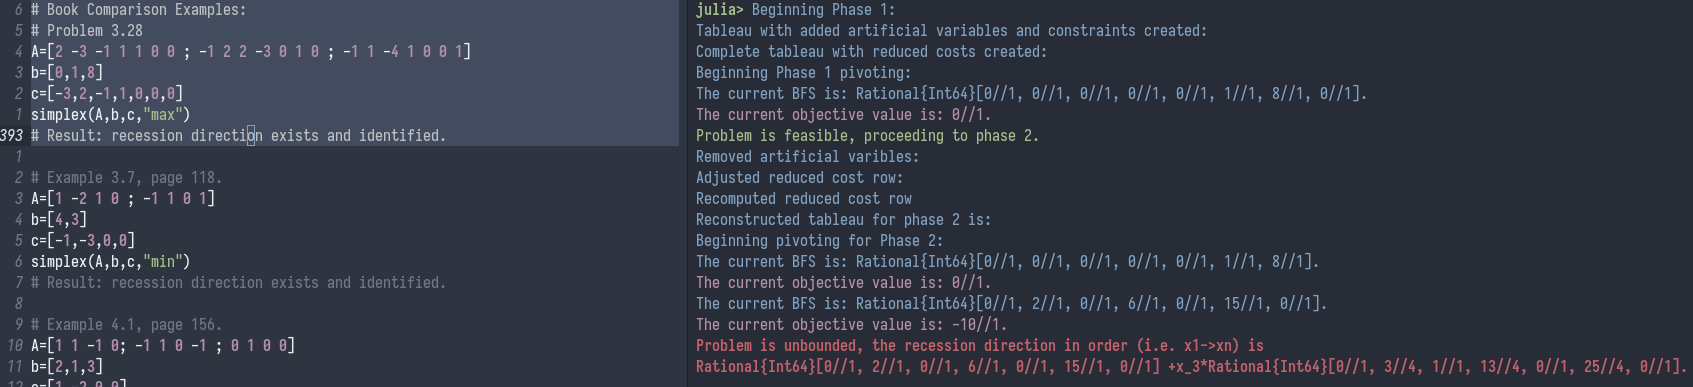
\includegraphics[width=1\textwidth]{figure1.png}\\
Test 1 for unboundedness $\uparrow$\\

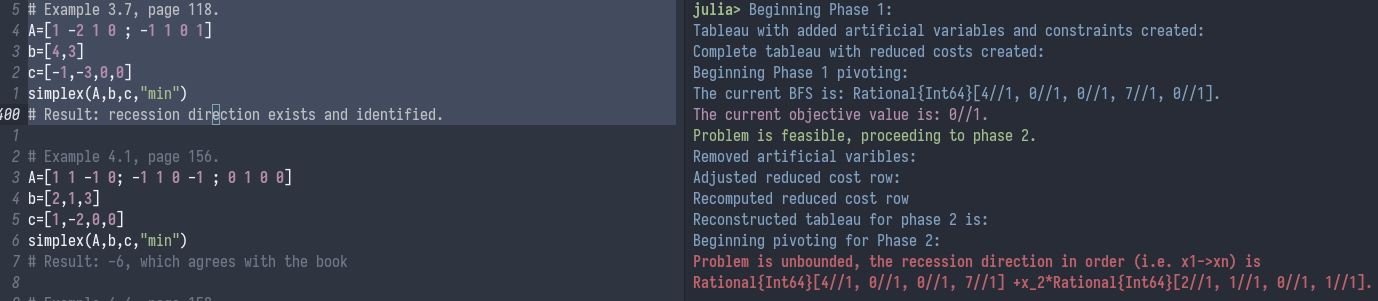
\includegraphics[width=\textwidth]{figure2.png}\\
Test 2 for unboundedness $\uparrow$\\

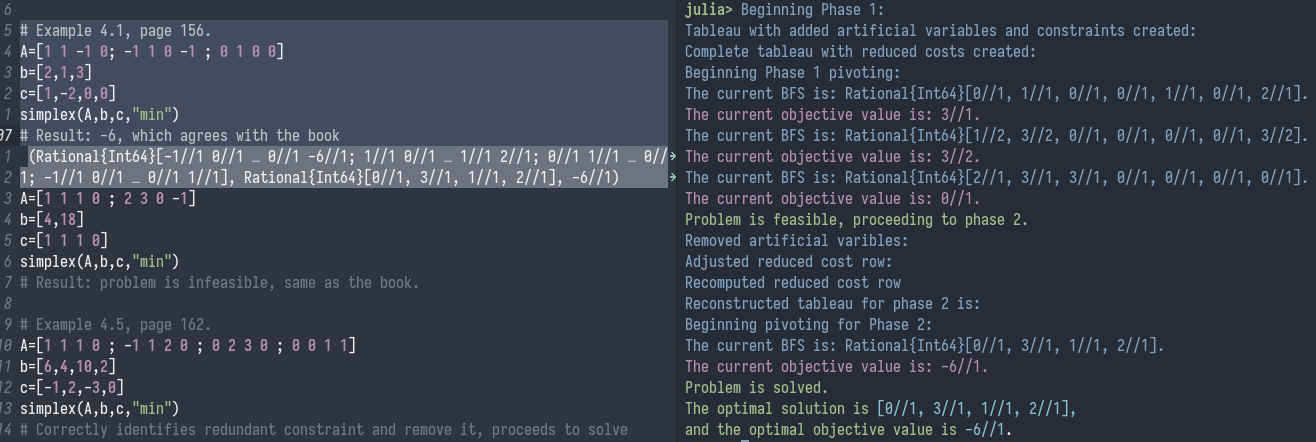
\includegraphics[width=\textwidth]{figure3.png}\\
Test 1 for optimal solution $\uparrow$\\

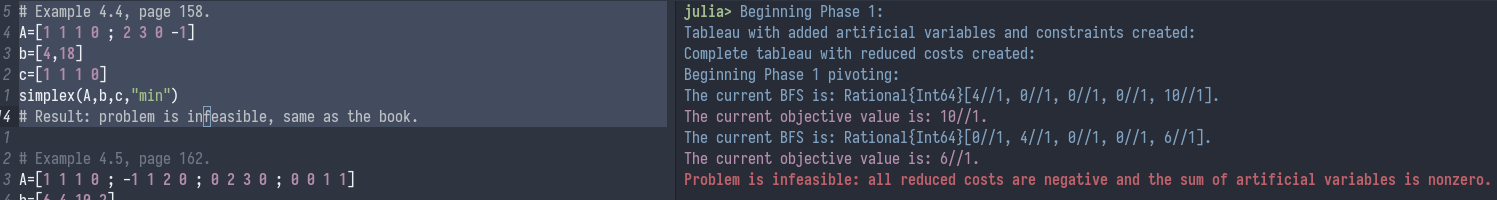
\includegraphics[width=\textwidth]{figure4.png}\\
Test 1 for infeasibility $\uparrow$\\

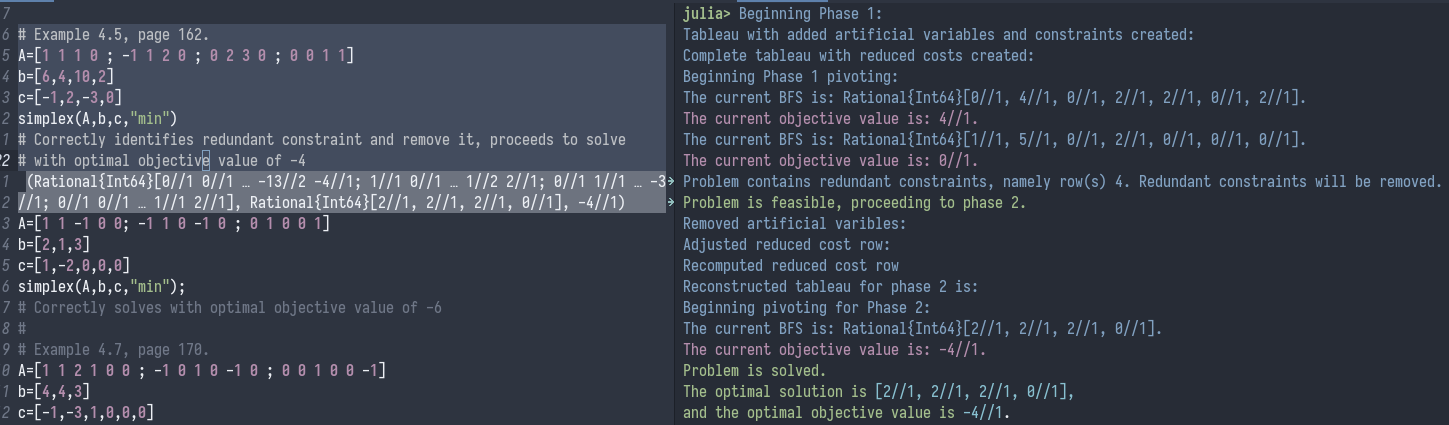
\includegraphics[width=\textwidth]{figure5.png}\\
Test 2 for optimal solution $\uparrow$\\

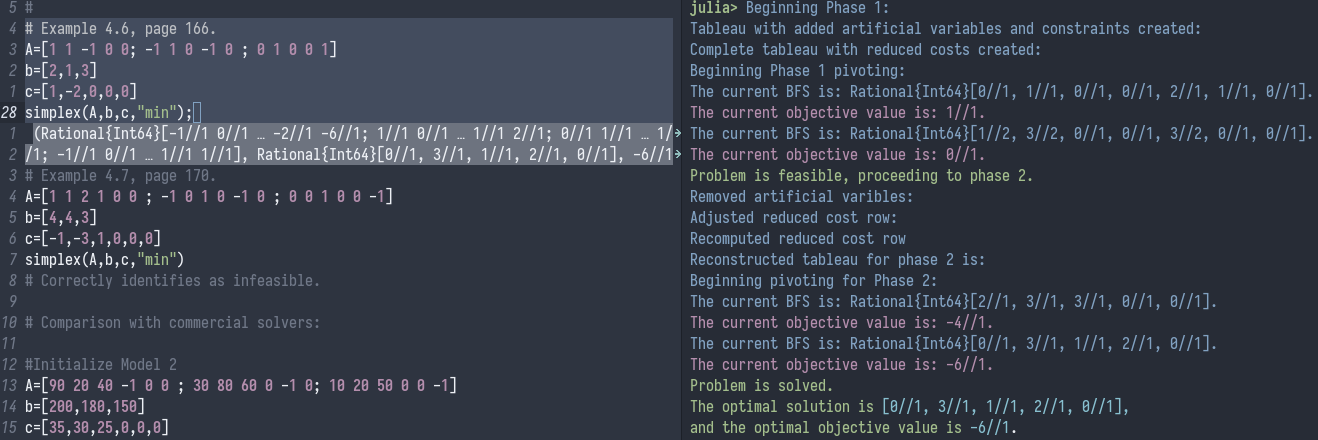
\includegraphics[width=\textwidth]{figure6.png}\\
Test 3 for optimal solution $\uparrow$\\

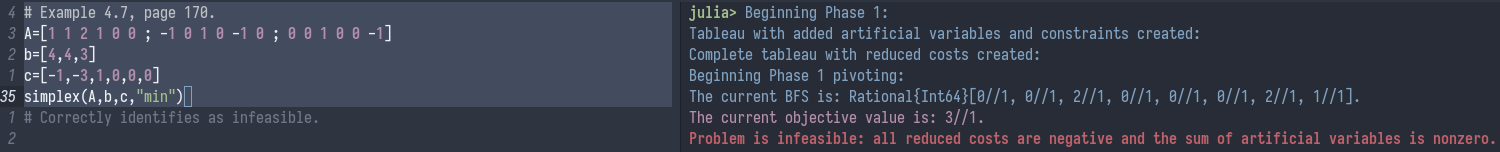
\includegraphics[width=\textwidth]{figure7.png}\\
Test 2 for infeasibility $\uparrow$
\end{center}
\section{Performance Evaluation}
\label{sec:org26e9204}
\subsection{Problem 2 Code}
\label{sec:org528cab0}
\subsubsection{Problem Formulation}
\label{sec:org761ff96}
See formulation above in the introduction \ref{sec:org9d5c16c}.
\subsubsection{Code}
\label{sec:org50415e9}
\begin{minted}[,julia]{julia}
# Comparison with commercial solvers:

#Initialize Model 2
A=[90 20 40 -1 0 0 ; 30 80 60 0 -1 0; 10 20 50 0 0 -1]
b=[200,180,150]
c=[35,30,25,0,0,0]
model=Model(HiGHS.Optimizer)
set_optimizer_attribute(model, "presolve", "off")
# Define decision variables
@variable(model, x[1:6]);
# Add constraints (in  this case simple matrix based ones)
# Note for problem 1 I need to double check I didn't transpose the A matrix incorrectly.
@constraint(model, A*x .== b );
@constraint(model, x .>= Rational.(zeros(6)) );
# Define the objective function
@objective(model, Min, c'*x);
# Optimize the model
optimize!(model)
res=simplex(A,b,c,"min");
if(raw_status(model) == "kHighsModelStatusOptimal")
    # Check if my model is sufficiently close to the HiGHS optimizer
    # note mine should be correct as I'm using rational arithemetic, with
    # unlimited precision, not floating point values.
    if(isapprox(res[3],objective_value(model),rtol=0.0001))
        printstyled("Success: Models are sufficiently close!\n",color=:green)
    else
        printstyled("Failure: Models are NOT sufficiently close!\n",color=:red)
    end
elseif(res==nothing)
        printstyled("Success: Both show unboundedness
                               or infeasibility!",color=:green)
else
        printstyled("Failure: My algorithm disagrees with HiGHS.)",color=:red)
end

\end{minted}

\subsubsection{Screenshots of Evaluation and Results}
\label{sec:orga6cab65}

\begin{center}
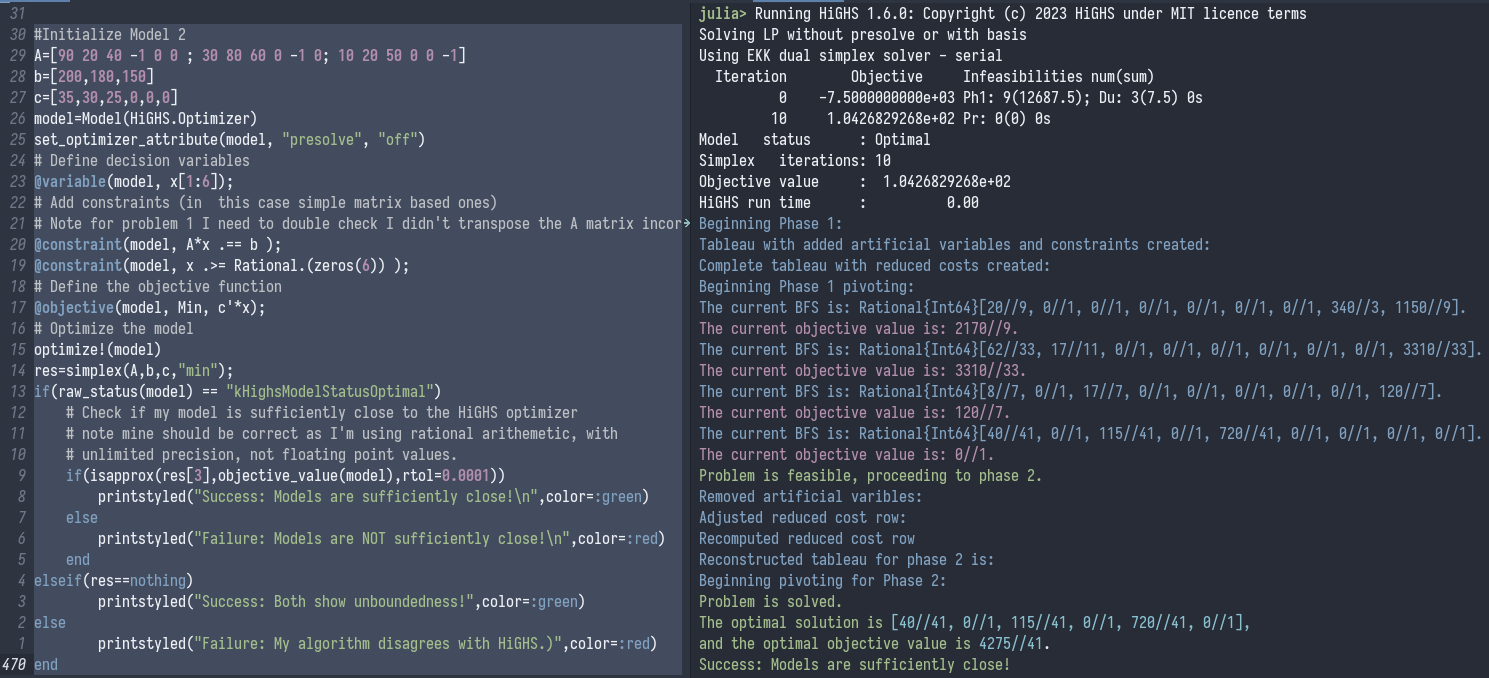
\includegraphics[width=1\textwidth]{figure8.png}\\
Comparison of my solver with JuMP+HiGHS for problem 2 which also includes my testing code to compare the outputs. Note that the bottom line of the right panel in the screenshot indicates my model agrees with HiGHS\\
\end{center}

\vfill
Please continue to next page
\newpage

\subsection{Problem 16 Code}
\label{sec:org203be40}
See formulation above in the introduction \ref{sec:org418163d}.

\begin{minted}[,julia]{julia}
#Initialize Model 16

# Note, these constructions look strange due to the
# fraction -> float -> rational conversion
# normally my code handles everything well
# but occasionally I had to do this due to Julia's
# limitations.
A=vcat(Rational.(
 [1 0 0 1 0 0 1 0 0 1 0 0 0 0 0 0 0 0;
   0 1 0 0 1 0 0 1 0 0 1 0 0 0 0 0 0 0;
   0 0 1 0 0 1 0 0 1 0 0 1 0 0 0 0 0 0;
   20 0 0 15 0 0 12 0 0 0 0 0 1 0 0 0 0 0;
   0 20 0 0 15 0 0 12 0 0 0 0 0 1 0 0 0 0;
   0 0 20 0 0 15 0 0 12 0 0 0 0 0 1 0 0 0;
   1 1 1 0 0 0 0 0 0 0 0 0 0 0 0 1 0 0;
   0 0 0 1 1 1 0 0 0 0 0 0 0 0 0 0 1 0;
   0 0 0 0 0 0 1 1 1 0 0 0 0 0 0 0 0 1]),
   Rational.( [1//750 -1//900 0//1 1//750 -1//900 0//1 1//750 -1//900 0 0 0 0 0 0 0 0 0 0]),
   Rational.( [1//750 0//1 -1//450 1//750 0//1 -1//450 1//750 0//1 -1//450  0 0 0 0 0 0 0 0 0]))
b=[750,900,450,13000,12000,5000,900,1200,750,0,0]
c=vcat([385,385,385,330,330,300,275,275,275],zeros(9))
model=Model(HiGHS.Optimizer)
set_optimizer_attribute(model, "presolve", "off")
# Define decision variables
@variable(model, x[1:18]);
# Add constraints (in  this case simple matrix based ones)
# Note for problem 1 I need to double check I didn't transpose the A matrix incorrectly.
@constraint(model, A*x .== b );
@constraint(model, x .>= Rational.(zeros(18)) );
# Define the objective function
@objective(model, Max, c'*x);
# Optimize the model
optimize!(model)
#Run my simplex algorithm
res=simplex(A,b,c,"max");
if(raw_status(model) == "kHighsModelStatusOptimal")
    # Check if my model is sufficiently close to the HiGHS optimizer
    # note mine should be correct as I'm using rational arithemetic, with
    # unlimited precision, not floating point values.
    if(isapprox(res[3],objective_value(model),rtol=0.0001))
        printstyled("Success: Models are sufficiently close!\n",color=:green)
    else
        printstyled("Failure: Models are NOT sufficiently close!\n",color=:red)
    end
elseif(res==nothing)
        printstyled("Success: Both show
                              unboundedness or infeasibility!",color=:green)
else
        printstyled("Failure: mine doesn't agree with HiGHS.",color=:red)
end
\end{minted}

\subsubsection{Screenshots of Evaluation and Results}
\label{sec:orgd3c49cc}
\begin{center}
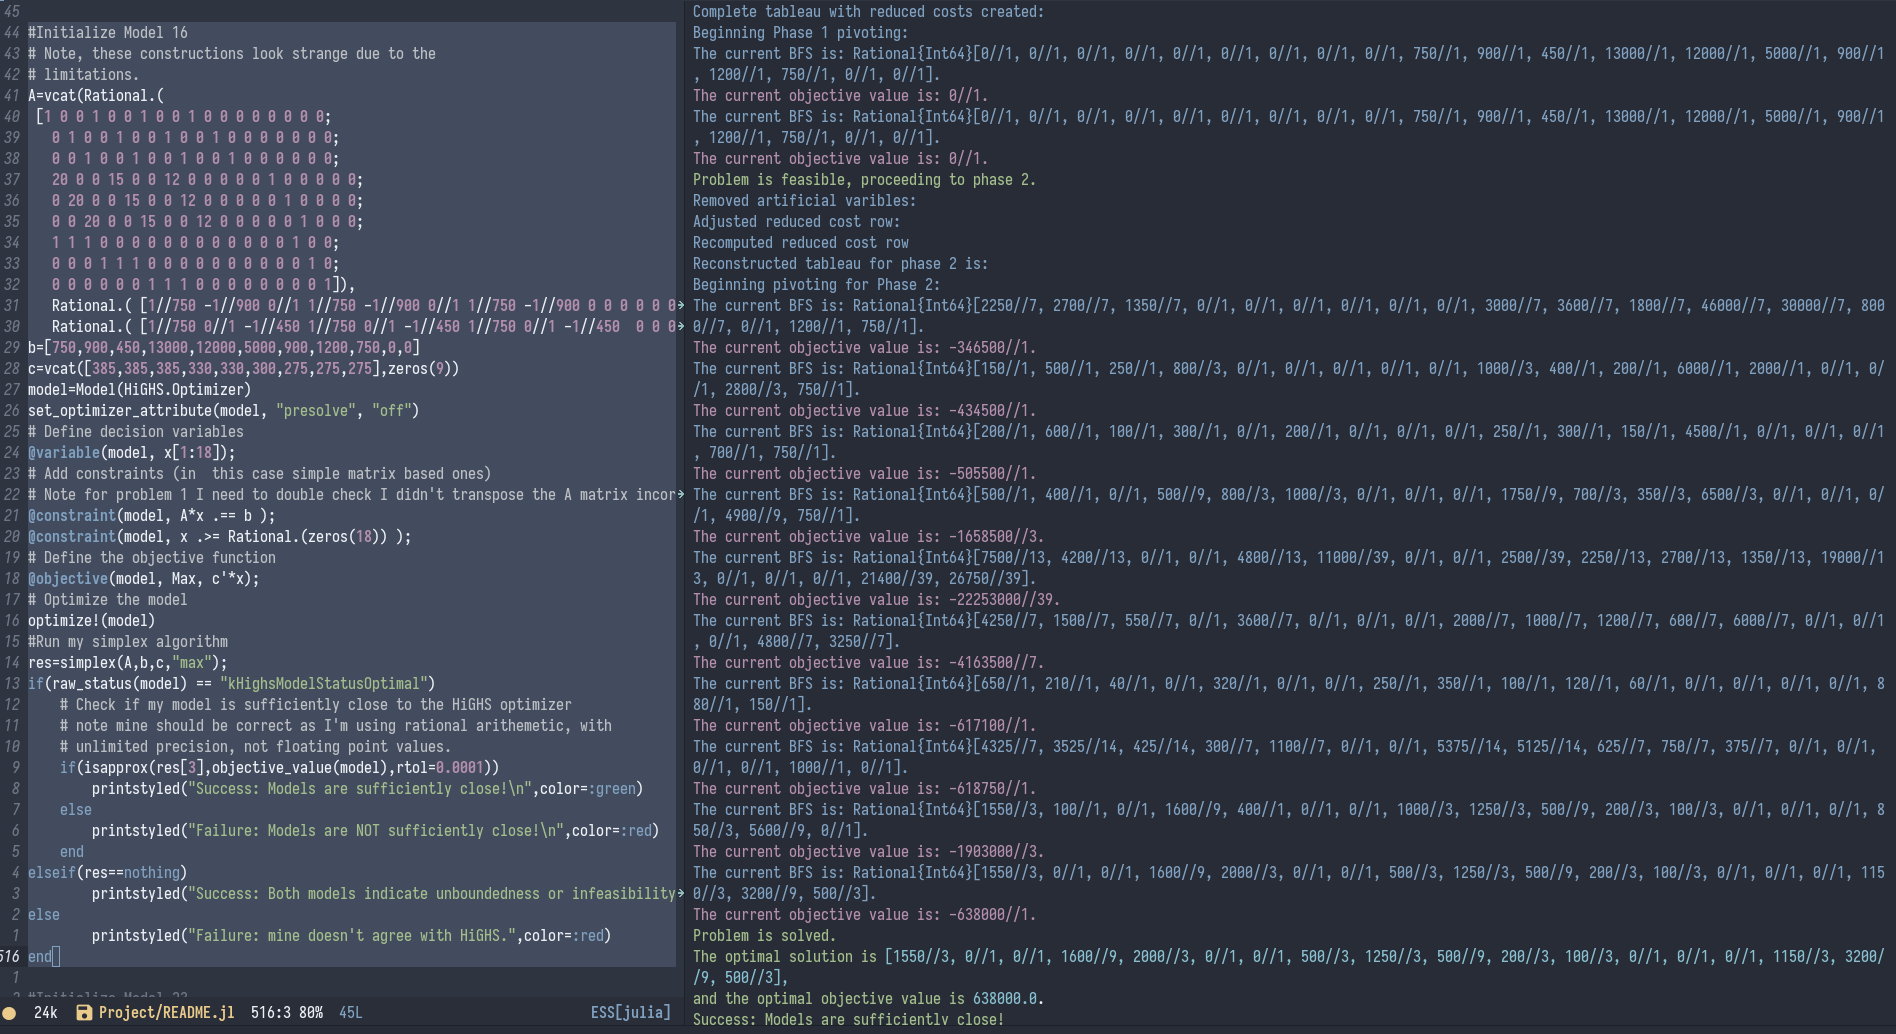
\includegraphics[width=1\textwidth]{figure9.png}\\
Comparison of my solver with JuMP+HiGHS for problem 16 which also includes my testing code to compare the outputs. Note that the bottom line of the right panel in the screenshot indicates my model agrees with HiGHS. Apologies for the large volume of output, but this one shows that the complete tabluea in phase 1 was completed, all the way to the end of phase 2.
\end{center}


\vfill
Please continue to next page
\newpage

\subsection{Problem 23 Code}
\label{sec:org3cb218a}
See formulation above in \ref{sec:orgfe951c7}.
\begin{minted}[,julia]{julia}
#Initialize Model 23
model=Model(HiGHS.Optimizer)
set_optimizer_attribute(model, "presolve", "off")
@variable(model, x[1:14]);
@constraint(model, ([9,6,8.5,12,3.5,16,16,26,24,41,34,45,0,0]./100)' *x >= 0.2);
@constraint(model, ([0.5,3,4,4.5,0,4,4,8.5,2,1.5,1,0.5,0,0]./100)' *x >= 0.03);
@constraint(model, ([20,16,2.5,12,0,8,10.5,9,8,13,8,6.5,0,0]./100)' *x <= 0.12);
@constraint(model, 0.01 <= ([0.7,2,0.02,0.1,0.6,0.1,0.1,0.15,
                             0.3,0.1,0.35,0.2,36,32]./100)' *x <= 0.02);
@constraint(model, 0.006 <= ([0.05,0.1,0.25,0.4,0.1,0.9,1.2,
                              0.6,0.65,1.2,0.8,0.6,0.5,14]./100)' *x <= 0.02);

@constraint(model, ([0.7,2,0.02,0.1,0.6,0.1,0.1,0.15,0.3,0.1,0.35,0.2,36,32]./100
.- [0.05,0.1,0.25,0.4,0.1,0.9,1.2,0.6,0.65,1.2,0.8,0.6,0.5,14]./100)' *x >= 0);

@constraint(model, x.>= [4,1,1,1,5,5,5,5,1,1,1,1,0,1]./100);
@constraint(model, x.<= [20,20,25,25,14,30,30,15,25,35,35,35,2,2]./100);
@constraint(model, sum(x) == 1);
@constraint(model, 0.05 <= x[1]+x[2]<= 0.20);
@constraint(model, 0.20 <= x[3]+x[4]<= 0.35);
@constraint(model, 0.10 <= x[6]+x[7]<= 0.30);
@constraint(model, 0.02 <= x[8]+x[9]<= 0.25);
@constraint(model, 0.03 <= x[10]+x[11]+x[12]<= 0.35);
@objective(model, Min, [64,35,55,54,19,64,62,77,66,74,85,108,10,66]'*x);
# Optimize the model
optimize!(model)
obj=objective_value(model)

# This problem was so large and cumbersome I had to write the values for A and b
# in a csv file to make sure I wasn't getting any typos. I knew the mistake was with
# my model and not the code because I was able to test the constraint matrices
# in HiGHS as well which got the same (wrong) result as my model. Hence why
# I'm importing them from a CSV.
A=readdlm("test2.csv", ',', String)
A=Meta.parse.(A)
A=eval.(A)
A=Rational.(A)
b=A[:,end]
A=A[:,1:end-1]
c=vcat(Rational.([64,35,55,54,19,64,62,77,66,74,85,108,10,66]),Rational.(zeros(60-14)))

# Sanity check
model=Model(HiGHS.Optimizer)
set_optimizer_attribute(model, "presolve", "off")
@variable(model, x[1:60]);
# Add constraints (in  this case simple matrix based ones)
# Note for problem 1 I need to double check I didn't transpose the A matrix incorrectly.
@constraint(model, A*x .== b );
@constraint(model, x .>= 0 );
# Define the objective function
@objective(model, Min, c'*x);
# Optimize the model
optimize!(model)
println("Original model and the matrix form perform the same?",obj==objective_value(model))
#Run my simplex algorithm
res=simplex(A,b,c,"min");
if(raw_status(model) == "kHighsModelStatusOptimal")
    # Check if my model is sufficiently close to the HiGHS optimizer
    # note mine should be correct as I'm using rational arithemetic, with
    # unlimited precision, not floating point values.
    if(isapprox(res[3],objective_value(model),rtol=0.0001))
        printstyled("Success: Models are sufficiently close!\n",color=:green)
    else
        printstyled("Failure: Models are NOT sufficiently close!\n",color=:red)
    end
elseif(res==nothing)
        printstyled("Success: Both show
                               unboundedness or infeasibility!",color=:green)
else
        printstyled("Failure: mine doesn't agree with HiGHS.",color=:red)
end
\end{minted}

\subsubsection{Screenshots of Evaluation and Results}
\label{sec:org13dabec}
\begin{center}
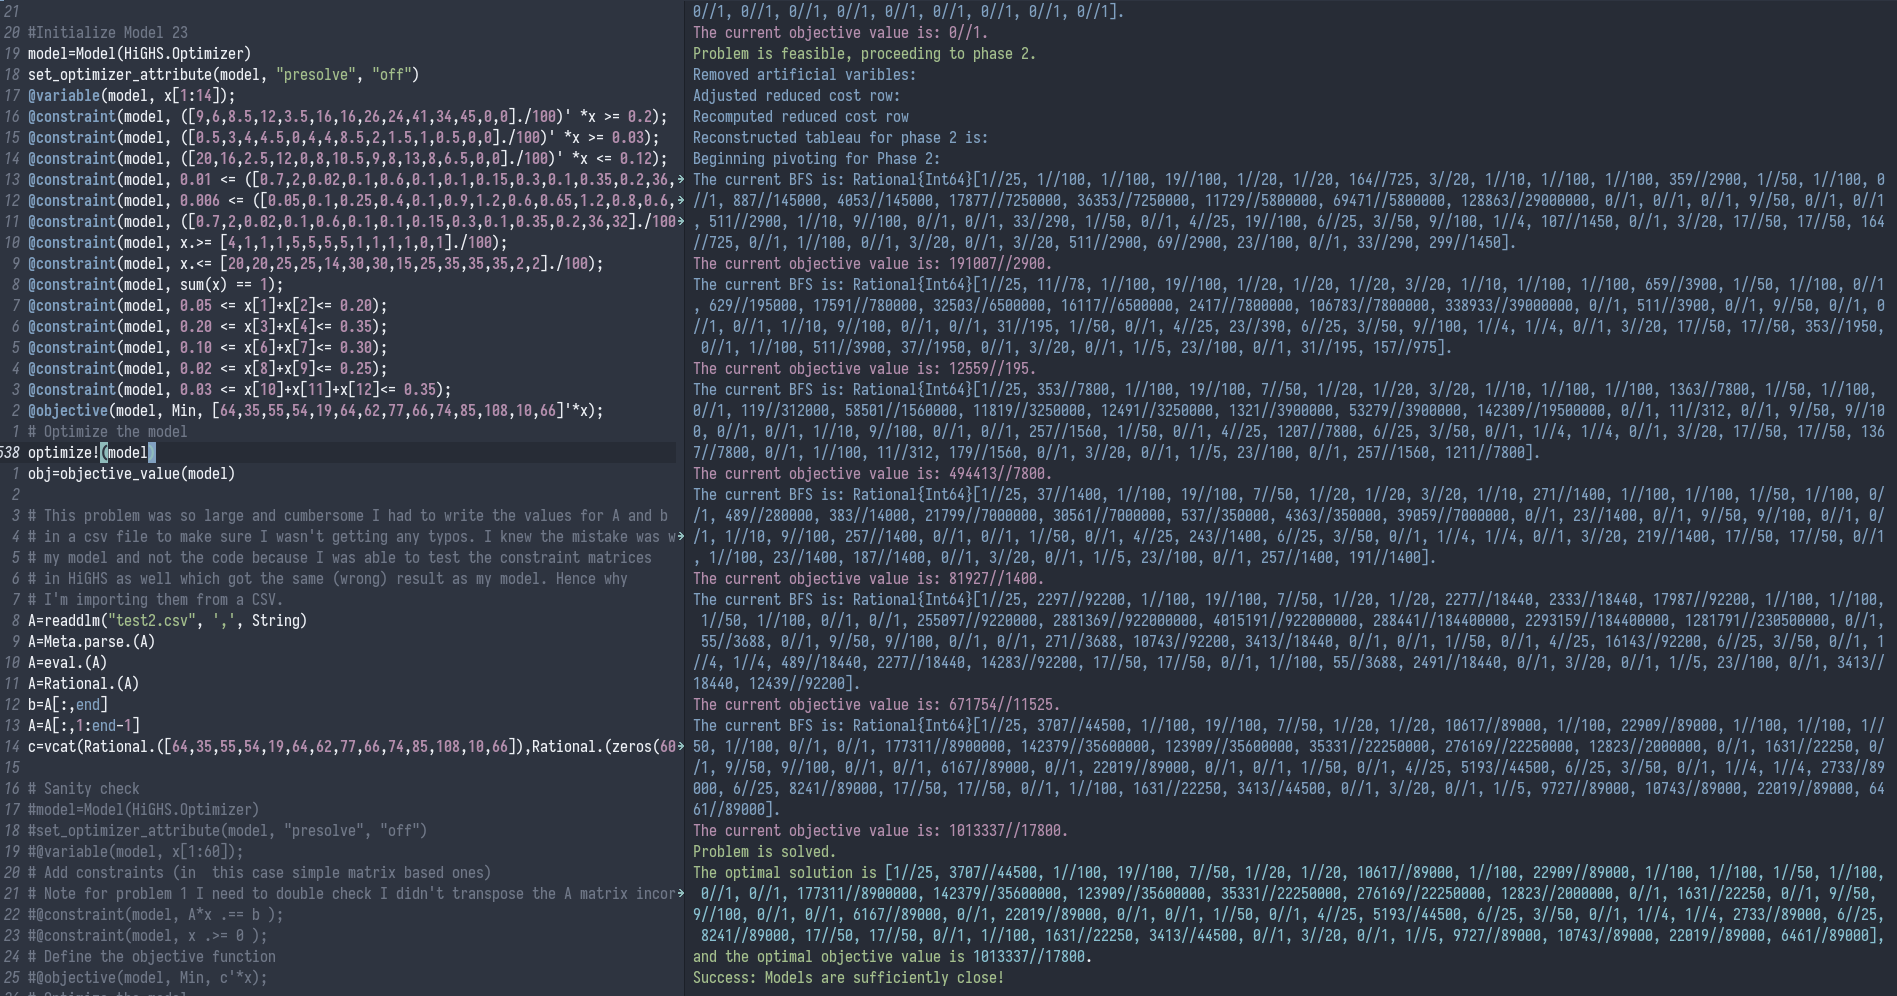
\includegraphics[width=1\textwidth]{figure10.png}\\
Comparison of my solver with JuMP+HiGHS for problem $23^{*}$ which also includes my testing code to compare the outputs. Note that the bottom line of the right panel in the screenshot indicates my model agrees with HiGHS. Apologies for even more output, but this problem was massive which made the BFS solutions quite long. This screenshot only shows that the last pivot of phase 1 resulted in a feasible tableau, and then all of phase 2's outputs were recorded as well.
\end{center}
\end{document}